


\tikzset{every picture/.style={line width=0.75pt}} %set default line width to 0.75pt        

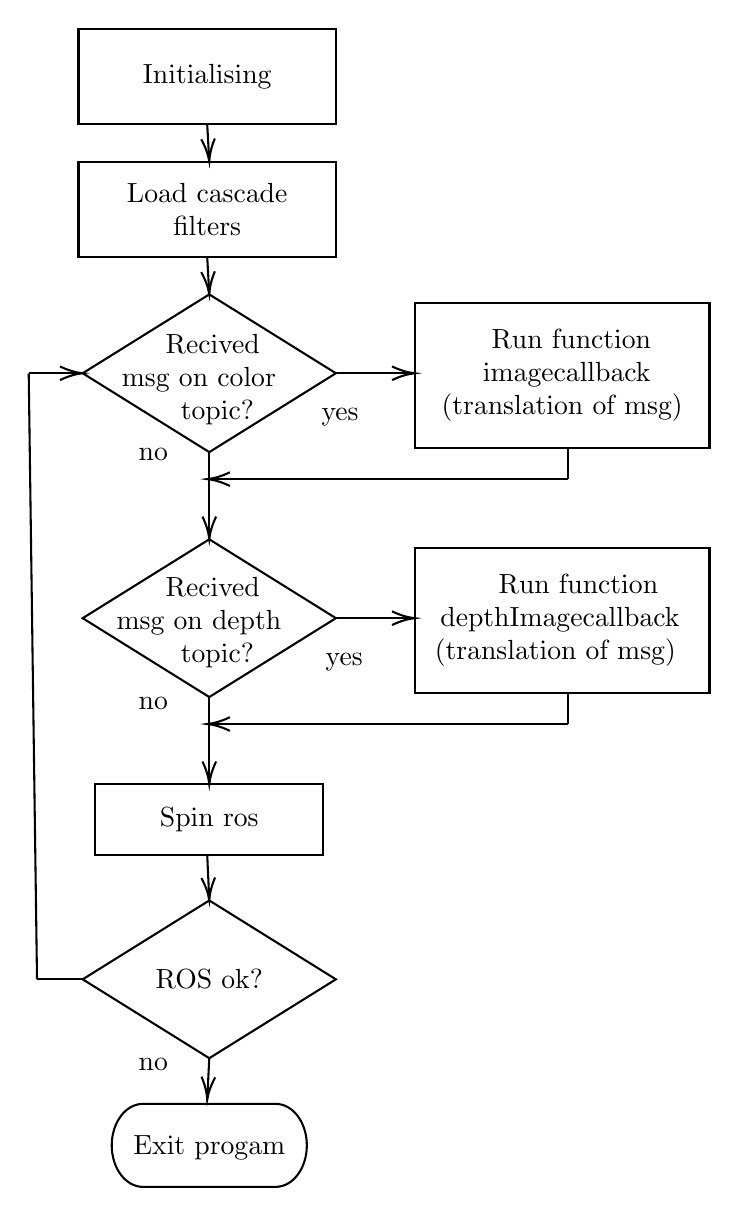
\begin{tikzpicture}[x=0.75pt,y=0.75pt,yscale=-1,xscale=1]
%uncomment if require: \path (0,571.2999877929688); %set diagram left start at 0, and has height of 571.2999877929688

%Flowchart: Process [id:dp9246505832510836] 
\draw   (30,70) -- (154,70) -- (154,116) -- (30,116) -- cycle ;
%Flowchart: Decision [id:dp5687244167692472] 
\draw   (93,134) -- (154,172) -- (93,210) -- (32,172) -- cycle ;
%Straight Lines [id:da310436632905724] 
\draw    (92,116) -- (92.89,132) ;
\draw [shift={(93,134)}, rotate = 266.82] [color={rgb, 255:red, 0; green, 0; blue, 0 }  ][line width=0.75]    (10.93,-3.29) .. controls (6.95,-1.4) and (3.31,-0.3) .. (0,0) .. controls (3.31,0.3) and (6.95,1.4) .. (10.93,3.29)   ;

%Straight Lines [id:da9071987627299013] 
\draw    (154,172) -- (190,172) ;
\draw [shift={(192,172)}, rotate = 180] [color={rgb, 255:red, 0; green, 0; blue, 0 }  ][line width=0.75]    (10.93,-3.29) .. controls (6.95,-1.4) and (3.31,-0.3) .. (0,0) .. controls (3.31,0.3) and (6.95,1.4) .. (10.93,3.29)   ;

%Flowchart: Process [id:dp3608842236348597] 
\draw   (192,138) -- (334,138) -- (334,208) -- (192,208) -- cycle ;
%Flowchart: Decision [id:dp4580696844035561] 
\draw   (93,252) -- (154,290) -- (93,328) -- (32,290) -- cycle ;
%Straight Lines [id:da16050336544145083] 
\draw    (154,290) -- (190,290) ;
\draw [shift={(192,290)}, rotate = 180] [color={rgb, 255:red, 0; green, 0; blue, 0 }  ][line width=0.75]    (10.93,-3.29) .. controls (6.95,-1.4) and (3.31,-0.3) .. (0,0) .. controls (3.31,0.3) and (6.95,1.4) .. (10.93,3.29)   ;

%Flowchart: Process [id:dp871969364959173] 
\draw   (192,256) -- (334,256) -- (334,326) -- (192,326) -- cycle ;
%Straight Lines [id:da34598842864976675] 
\draw    (93,210) -- (93,250) ;
\draw [shift={(93,252)}, rotate = 270] [color={rgb, 255:red, 0; green, 0; blue, 0 }  ][line width=0.75]    (10.93,-3.29) .. controls (6.95,-1.4) and (3.31,-0.3) .. (0,0) .. controls (3.31,0.3) and (6.95,1.4) .. (10.93,3.29)   ;

%Straight Lines [id:da833074157082355] 
\draw    (266,208) -- (266,223) ;


%Straight Lines [id:da42041676547080575] 
\draw    (266,223) -- (94,223) ;
\draw [shift={(92,223)}, rotate = 360] [color={rgb, 255:red, 0; green, 0; blue, 0 }  ][line width=0.75]    (10.93,-3.29) .. controls (6.95,-1.4) and (3.31,-0.3) .. (0,0) .. controls (3.31,0.3) and (6.95,1.4) .. (10.93,3.29)   ;

%Straight Lines [id:da2386232122180666] 
\draw    (93,328) -- (93,368) ;
\draw [shift={(93,370)}, rotate = 270] [color={rgb, 255:red, 0; green, 0; blue, 0 }  ][line width=0.75]    (10.93,-3.29) .. controls (6.95,-1.4) and (3.31,-0.3) .. (0,0) .. controls (3.31,0.3) and (6.95,1.4) .. (10.93,3.29)   ;

%Straight Lines [id:da728184268688258] 
\draw    (266,326) -- (266,341) ;


%Straight Lines [id:da460556600018038] 
\draw    (266,341) -- (94,341) ;
\draw [shift={(92,341)}, rotate = 360] [color={rgb, 255:red, 0; green, 0; blue, 0 }  ][line width=0.75]    (10.93,-3.29) .. controls (6.95,-1.4) and (3.31,-0.3) .. (0,0) .. controls (3.31,0.3) and (6.95,1.4) .. (10.93,3.29)   ;

%Flowchart: Process [id:dp1957870496926526] 
\draw   (38,370) -- (148,370) -- (148,404) -- (38,404) -- cycle ;
%Flowchart: Decision [id:dp5537528056529856] 
\draw   (93,426) -- (154,464) -- (93,502) -- (32,464) -- cycle ;
%Straight Lines [id:da7922304652544767] 
\draw    (92,404) -- (92.91,424) ;
\draw [shift={(93,426)}, rotate = 267.4] [color={rgb, 255:red, 0; green, 0; blue, 0 }  ][line width=0.75]    (10.93,-3.29) .. controls (6.95,-1.4) and (3.31,-0.3) .. (0,0) .. controls (3.31,0.3) and (6.95,1.4) .. (10.93,3.29)   ;

%Straight Lines [id:da8067244819945293] 
\draw    (6,172) -- (30,172) ;
\draw [shift={(32,172)}, rotate = 180] [color={rgb, 255:red, 0; green, 0; blue, 0 }  ][line width=0.75]    (10.93,-3.29) .. controls (6.95,-1.4) and (3.31,-0.3) .. (0,0) .. controls (3.31,0.3) and (6.95,1.4) .. (10.93,3.29)   ;

%Straight Lines [id:da7906439890089335] 
\draw    (6,172) -- (10,464) ;


%Straight Lines [id:da4724416457043301] 
\draw    (10,464) -- (32,464) ;


%Flowchart: Terminator [id:dp37784648805984133] 
\draw   (61.04,524) -- (124.96,524) .. controls (133.27,524) and (140,532.95) .. (140,544) .. controls (140,555.05) and (133.27,564) .. (124.96,564) -- (61.04,564) .. controls (52.73,564) and (46,555.05) .. (46,544) .. controls (46,532.95) and (52.73,524) .. (61.04,524) -- cycle ;
%Straight Lines [id:da6901416867506117] 
\draw    (93,502) -- (92.1,520) ;
\draw [shift={(92,522)}, rotate = 272.86] [color={rgb, 255:red, 0; green, 0; blue, 0 }  ][line width=0.75]    (10.93,-3.29) .. controls (6.95,-1.4) and (3.31,-0.3) .. (0,0) .. controls (3.31,0.3) and (6.95,1.4) .. (10.93,3.29)   ;

%Flowchart: Process [id:dp1779072269358366] 
\draw   (30,6) -- (154,6) -- (154,52) -- (30,52) -- cycle ;
%Straight Lines [id:da6425386329539113] 
\draw    (92,52) -- (92.89,68) ;
\draw [shift={(93,70)}, rotate = 266.82] [color={rgb, 255:red, 0; green, 0; blue, 0 }  ][line width=0.75]    (10.93,-3.29) .. controls (6.95,-1.4) and (3.31,-0.3) .. (0,0) .. controls (3.31,0.3) and (6.95,1.4) .. (10.93,3.29)   ;


% Text Node
\draw (92,93) node  [align=center] {Load cascade\\  filters};
% Text Node
\draw (88,175) node  [align=center] { \ \ \   Recived \\ msg on color\\ \ \ \ \  topic?};
% Text Node
\draw (263,173) node  [align=center] {\ \ Run function \\ \ imagecallback\\(translation of msg)};
% Text Node
\draw (88,292) node  [align=center] { \ \ \ Recived \\msg on depth\\ \ \ \ \ topic?};
% Text Node
\draw (257.5,291) node  [align=center] { \ \ \ \ \ \ Run function \\ \ \ depthImagecallback\\ \ (translation of msg)};
% Text Node
\draw (93,387) node  [align=left] {Spin ros};
% Text Node
\draw (93,464) node  [align=left] {ROS ok?};
% Text Node
\draw (93,545) node  [align=left] {Exit progam};
% Text Node
\draw (66,211) node  [align=left] {no};
% Text Node
\draw (66,331) node  [align=left] {no};
% Text Node
\draw (66,505) node  [align=left] {no};
% Text Node
\draw (156,193) node  [align=left] {yes};
% Text Node
\draw (158,311) node  [align=left] {yes};
% Text Node
\draw (92,29) node  [align=left] { Initialising};


\end{tikzpicture}





